\documentclass[oneside, 11pt]{book}
\usepackage[titletoc]{appendix}
\usepackage{geometry}
\usepackage{natbib}
\usepackage{epsfig}
%\usepackage{hyperref}
\usepackage{upgreek}
\usepackage{bbold}
\usepackage[english]{babel}
\usepackage[applemac]{inputenc}
\usepackage{setspace}
\usepackage{caption}
\usepackage{amsthm}
\usepackage{float}
\usepackage{placeins}
\usepackage{natbib}
\usepackage{amsmath,amsfonts,amsthm,amssymb}
\usepackage{url}
\usepackage{multirow}
\usepackage{subfigure}
\usepackage{algorithm}
\usepackage[noend]{algpseudocode}
\newtheorem{mydef}{Definition}
\onehalfspacing
\makeatletter
\def\url@leostyle{%
  \@ifundefined{selectfont}{\def\UrlFont{\sf}}{\def\UrlFont{\small\ttfamily}}}
\makeatother
\geometry{a4paper,left=24mm,right=24mm, top=33mm, bottom=3.1cm}
\urlstyle{leo}
\usepackage{fancyhdr}
\pagestyle{fancy}
\fancyhf{}
\fancyhead[C]{Active Sampling as Bayesian Quadrature}
\fancyfoot[C]{ \thepage}

\begin{document}


\newcommand{\hmwkCourse}{MSc Cognitive and Decision Sciences\vspace{18mm}}
\newcommand{\hmwkTitle}{{\bf Active Sampling as Sequential Bayesian Quadrature} \vspace{18mm} \\ 
Master of Science -Thesis}
\newcommand{\hmwkSubTitle}{} % No subtitle, so this will be excluded
\newcommand{\hmwkDueDate}{\today}
\newcommand{\hmwkClassInstructor}{}
\newcommand{\hmwkAuthorName}{Christoph Niemeyer}
\newcommand{\LastPage}{TBA}

\begin{titlepage}
\vspace{20mm}
\begin{center}
\vspace{150mm}
\LARGE{ UNIVERSITY COLLEGE LONDON \\ \hmwkCourse \\[6.5cm]

\includegraphics[width=4cm]{ucl.jpg}\\
\vspace{-110mm}
 {\hmwkTitle}  \\}
\vspace{80mm}
\Large Submission for Candidate:\\
Christoph Niemeyer\\
Department of Experimental Psychology
\\
\Large \today\vspace{28mm} \\ 
\begin{tabular}{ll}
Primary Supervisor:&Eric Schulz\\
Second Grader: &Maarten Speekenbrink
\end{tabular}
\end{center}
\end{titlepage}
\vspace*{1cm}
\begin{center}
\textbf{{\LARGE Declaration of Authorship:}}\\
\end{center}
\vspace{1cm}
\begin{enumerate}
\item I am aware of the University's disciplinary regulations concerning conduct in examinations and, in particular, of the regulations on plagiarism.
\item The thesis work I am submitting is entirely my own work except where otherwise indicated.
\item This thesis has not been submitted, either wholly or substantially, for another degree of this University, or for a degree at any other institution.
\item I have clearly signaled the presence of quoted or paraphrased material and referenced all sources.
\item I have acknowledged appropriately any assistance I have received in addition to that provided by my supervisor.
\item I have not sought assistance from any professional agency. 
\end{enumerate}
\vspace{2cm}
\begin{center}
Christoph Niemeyer, \today
\end{center}
\newpage
\begin{center}
\textbf{{\LARGE Abstract:}}\\
\end{center}
How can and should an agent actively learn about probability distributions? Psychological theories involving sampling are vast, but currently there is no real theory about how humans actively acquire knowledge about explicit probability distributions. The thesis at hand therefore tries to develop a theory of active sampling based on \emph{Gaussian Processes Quadrature}, a non-parametric class of density estimation.\\
The thesis will first summarize current psychological theories about human sampling and then introduce Gaussian Processes as an approach to Quadrature. It will be shown how Gaussian processes can be used to explore any probability distribution.\\
Multiple different sampling metaphors will be stated and all of them will be tested at how well they describe participants' active sampling behavior within a simple active density exploration task. Overall the Gaussian Process-based Quadrature approach will be shown to describe participants' behavior best.\\
The thesis will continue and define a rather new niche to compare different sampling models based on how well they can predict human active sampling behavior. Potential consequences and future experiments based on this assay will be examined.\\
Limitations and connections to related research questions will be discussed.\bigskip\\
\begin{center}
\textbf{KEYWORDS:} Active Sampling, Bayesian Quadrature, Gaussian Processes
\end{center}
\newpage
\vspace*{1cm}
\begin{center}
\textbf{{\LARGE Acknowledgements:}}\\
\end{center}
Thanks to Eric Schulz, you're a wonderful human being! Also, my parents are nice, too.
\newpage
%%%%%%%%%%%%%%%%%%%%%%%%%%%%%%%%%%%%%%%%%%%%%%%%%%%%%%%%%%%%%%%%%%%%%%%%%%%%%%%%%%%
\vspace*{10cm}
\begin{center}
\textbf{\Large{``I love the creativeness of raw sampling.''}} (Moreno about Depeche Mode)
\end{center}
\newpage
%%%%%%%%%%%%%%%%%%%%%%%%%%%%%%%%%%%%%%%%%%%%%%%%%%%%%%%%%%%%%%%%%%%%%%%%%%%%%%%%%%%
\tableofcontents
\newpage
%%%%%%%%%%%%%%%%%%%%%%%%%%%%%%%%%%%%%%%%%%%%%%%%%%%%%%%%%%%%%%%%%%%%%%%%%%%%%%%%%%%
\chapter{Introduction}
Imagine you are in your are preparing for a party and you want to find the song that best fits your mood. If your library consists only of 10 songs, the task seems relatively easy. You could listen to all of them and choose the one you think fits best. But let us imagine your library exists of 300 songs. To complicate thing more: How do you know the right song is even in your library? Maybe it is not, and you need to find it on Spotify, Soundcloud, or the like. To complicate things even further: as you are taking your time finding the right song, your mood will likely change. How do you go about finding the right song?\\
 
You could, of course, still simply choose a song at random. You might get a hit, but chances for that are very low. Should you rather choose one from your existing playlist only? You could listen to all 300 songs, but you would barely have time until the party starts. Perhaps there are queries you can ask to reduce your hypothesis space and improve your chances of getting a hit in time. For example, you may like to consider only those songs most recently played, the ones most often played, those that are not longer than three minutes etc. To complicate the example one last time: consider you do not have access to any technological device. Your search for a perfect song becomes a search for a perfect song in your mind. Undoubtedly, memory resources are now more restrained than in the case of an available computer aid. How does the brain guide memory searches? How does the brain decide, whether consciously or not, how much to think, when to stop thinking, or even what to think?\\

Examples of this sort highlight central questions in the study of intelligence. Recently, Gershman, Hovitz \& Tenenbaum (2015) reviewed central tendencies that arose in the fields of Artificial Intelligence, Cognitive Science and Neuroscience. These were seemingly divided at some point during the 1990s, focusing on different problems, mostly due to an increasing complexity in computer science and the focus on heuristics and biases in psychology. However, the authors argue that the two fields are re-converging, and this re-convergence is due to a large degree to the emergence of approximate inference methods coupled with smart Bayesian statistics. Approximate inference methods have enabled programs to cut down computational complexity, reducing the time it takes to make close to rational decisions, the cost associated with those decisions, and potentially to increase the benefits a decision can bring. \\
To many researchers, however, so-called Markov Chain Monte-Carlo (MCMC) methods have meant the biggest recent breakthrough in the study of intelligence from a Bayesian perspective. As many inference problems in Bayesian statistics are analytically intractable, the Bayesian approach came to a halt during a time when inference was almost always done in a strictly analytical sense. This, however, has changed completely with the emergence of MCMC based methods and an exponential increase of computational power over time. \\
The idea of a MCMC method is relatively simple: set up a Markov chain that is guaranteed to converge to an approximation of the target distribution over time and then use this approximation to perform tractable Bayesian inference. The popularity of these sampling mechanisms in statistics also influenced psychology during the recent years and many psychological theories these days are based on sampling assumptions, be it memory search, decision by sampling, or drift-diffusion models.\\
Crucially, however, most of these algorithms, in their traditional form, choose samples at random. Even though this theoretical choice does not influence the target distribution per se, it is a crucial assumption both statistically and psychologically considering the time until potential convergence is achieved. Coming back to the original example, if you want to find out what kind of songs you would like to listen to at a party, then sampling completely at random will most likely eat up a lot of time. Moreover, given a whole tradition of psychological experiments that show how participants do not behave randomly, but rather sample their environment actively by generating useful queries, a random sampling approach seems highly implausible.\\
Gladly, there exist more active methods to sample from probability distributions and perform inference at the same time. One such approach is called Bayesian Quadrature (henceforth BQ). BQ uses a probabilistic Bayesian Inference method based on Gaussian Process regression to estimate which site of a probability distribution is most likely of interest for the next sample in order to integrate over the probability space efficiently. The advantage of this method over conventional sampling approaches is striking. For one, it solves some decision problems with equal or better accuracy as Gaussian Processes can be seen as a universal function approximation engine that (in this case) can also approximate complex probability distributions. Most importantly however, it does not assume a completely random process to govern the search within the probability space and thus could potentially be the psychologically more plausible approach towards inference about probability densities. The likelihood of the data combined with prior information of it allows the system to make informed predictions at any point in time. This has the further advantage of explaining individual differences in decision strategies, given the data that has been observed thus far. Depending on perceived likelihood and prior information across machines or humans, predictions of potentially interesting samples will vary. Bayesian Quadrature is a viable candidate for probabilistic inferences in environments where uncertainty about states of the world is looming. And it is very well embedded in the literature of probabilistic inference mechanisms of the brain, giving additional power to those philosophers and scientists who support the metaphor of the ``brain as a machine''. Importantly, BQ also touches upon the debate of rationality. A machine's prediction is seen as rational given the data that informed it, although a prediction may not be accurate. With training, predictions can improve - rather than being deemed as irrational without hope of learning, as in the case of irrationality. This principle can also be applied to humans. Human behavior that diverges from normative models of utility, as most prominently demonstrated by research from Daniel Kahneman \& Amos Tversky (ref), is not irrational per se. Rather, differences in prior information, combined with a different perceived likelihood of the data, can explain why inaccurate predictions occur.\\

Surprisingly, however, this method has received very little attention from studies of actual human behavior and so most psychological studies on human sampling fall back on the overly simplistic assumption of random samples, with the exception of maybe MCMC with humans and some studies on mental rotation. The aim of this thesis, therefore, is to explore whether humans actively integrate information from a frequency distribution as predicted by Bayesian Quadrature or indeed sample completely at random. We develop a theory of active human sampling when the task is to judge about probabilities of events after a prior explicit sampling period. We argue that humans are not always sampling completely at random, but rather make sense of their environment by using highly adaptive and smartly designed sampling mechanisms, derived from a powerful Bayesian algorithm. \medskip\\

Chapter \S2 draws out a vision of a Bayesian Cognitivism and defines quadrature as an essential part of it. Chapter \S3 sets up the problem of quadrature and describes different sampling algorithms that have been proposed in the psychological literature as well as in statistical research. Chapter \S4, the methods section, sets up the design of the experiment and describes the participants in more detail. Chapter \S5 illustrates the results of the experiment and Chapter \S6 discusses potential problems, shortcomings, and future steps. Chapter \S7 will conclude the thesis by a call for more elaborate comparisons between different proposed sampling schemes.

%%%%%%%%%%%%%%%%%%%%%%%%%%%%%%%%%%%%%%%%%%%%%%%%%%%%%%%%%%%%%%%%%%%%%%%%%%%%%%%%%%%%%%%%%%%%%%%
\chapter{Bayesian Cognitivism}
\emph{This chapter will briefly describe a vision of Bayesian Cognitivism. Bayesian Cognitivism seeks out to model an intelligent system based on non-parametric Bayesian approaches that quantify uncertainty for each part. Quadrature is an important part thereof.}
\section{Cognitivism: Describing an intelligent system}
Cognitivism is a theoretical framework to understand how the mind works (ref). It makes two main claims: One, it holds that psychology can in principle be fully explained by the use of measurements and the scientific method (ref); Two, it holds that an intelligent system has internal mental states with representations and symbols, which can be manipulated by the use of rules or algorithms (ref). Cognitivism in itself, however, does not provide an explanation of how humans actually represent these internal states (ref). \\
Bayesian Cognitivism, as we call it, is an extension of traditional Cognitivism which at its fundaments uses Bayesian statistics and approximate inference methods to represent those internal mental states. In full, it is a computational framework that describes how an intelligent system can represent knowledge, make inferences, and learn.  To the best of our knowledge, it is the first attempt to explain uncertainty propagation and inference of an intelligent human system by the use of Bayesian statistics so far.\medskip\\
To understand the basic building blocks, let us describe Bayesian statistics before then explaining Bayesian Cognitivism.

\section{Probability Theory and Bayes rule}
There are two important rules to understand in probability theory:\\
First, the sum rule: 
\begin{align}
P(x) = \sum P(x,y)
\end{align}
Second, the product rule: 
\begin{align}
P(x,y) = P(x) P(y|x)
\end{align}

Here, $x$ and $y$ correspond to observed or uncertain quantities. For example, $x$ might relate to the weather in London and y might relate to the weather in Cambridge. $P(x)$ and $P(y)$ then correspond to the probability of $x$ or $y$ to be true, or the marginal probability. Note that these can be either a statement about the frequency of observing a particular value, as an objective measure, or a subjective belief about it, a term widely used in the psychological domain. $P(x,y)$ is the probability of the two events together, also the joint probability of observing $x$ and $y$. Importantly, $P(x|y)$ and $P(y|x)$ denote conditional probabilities, that is, the probability of $x$ given the observed value of $y$, and vice versa. For example, the probability of rain in London given that it is raining in Cambridge. The sum rule prescribes that the probability of $x$ is obtained by summing (or integrating for continuous variables) the joint probability over $y$. The product rule prescribes that we can decompose the joint probability as the product of the marginal and the conditional. Bayes rule follows from these two rules: 
\begin{align}
P(y|x) = \frac{(P(x|y) P(x))}{P(x)} = \frac{(P(x|y) P(y))} {\sum P(x,y)}
\end{align}

Machine learning makes use of these rules from probability theory to specify how a system learns. For that, we first need to replace some symbols: $x$ is replaced by $\mathcal{D}$ to denote the observed data; $y$ is replaced by $\theta$ to denote the unknown parameters of a model. Then, all terms are conditioned on a model $m$, which represents the class of probabilistic models under consideration. \\
Learning thus yields: 
\begin{align}
P(\theta |\mathcal{D},m) = \frac{(P(\mathcal{D}|\theta,m) P(\theta,m))}{P(\mathcal{D}|m)}
\end{align}
Here, $P(\mathcal{D}|\theta,m)$ is the likelihood of parameters $\theta$ in model $m$, $P(\theta|m)$ is the prior probability of $\theta$ and $P(\theta|\mathcal{D}, m)$ is the posterior of $\theta$ given data $\mathcal{D}$. For example, the data $\mathcal{D}$ might be a time series of hourly observations of the weather in Cambridge and London, and the model might attempt to capture the joint weather patterns at both locations over successive hours, with parameters $\theta$ modelling correlations over time and space. Learning, then, is the transformation of prior knowledge or assumptions about the parameters $P(\theta|m)$, through the data $\mathcal{D}$, into posterior knowledge about the parameters, $P(\theta|\mathcal{D},m)$. This posterior now becomes the prior to be used for future data. A learned model can be used to predict or forecast new unseen test data by simply applying the sum and product rule to get the prediction: 
\begin{align}
P(\mathcal{D}_{\text{test}}|\mathcal{D},m) = \int P(\mathcal{D}_{\text{test}}| \theta,\mathcal{D},m) P(\theta|\mathcal{D},m)d \theta
\end{align}
Finally, different models can be compared by applying Bayes rule at the level of $m$: 

\begin{align}
P(m|D) &= \frac{(P(\mathcal{D}| m) P(m))}{P(\mathcal{D})}\\
P(\mathcal{D}|m) &= \int P(\mathcal{D}| \theta ,m) P(\theta |m) d \theta
\end{align}
The term $P(\mathcal{D}|m)$ is then the marginal likelihood or model evidence - how likely the data is given a model.\medskip\\

Bayes rule and Probability Theory, as explained above, are the fundamentals upon which Bayesian Cognitivism is built. In theory, this is enough to explain how an agent can represent knowledge, make inferences, and learn. In practice, however, there are a number of modelling and computational challenges that narrow its applicability. One of the biggest challenges is what model to use in a Bayesian context and how to propagate uncertainty within a system.

\section{Gaussian Processes}
Gaussian Processes regression is a form f non-parametric Bayesian inference. It is a powerful approach that does not require us to choose the number of parameters or the shape of the function a priori, but rather lets the data speak by the means of Bayesian posterior calculations. As Gaussian Processes will be the workhorse for our Bayesian approach here, let us first define them mathematically before then outlining the Bayesian Cognitivism approach in more detail.\\
A Gaussian Process is a collection of random variables, any finite number of which have a joint Gaussian distribution. A $\mathcal{GP}$ is completely specified by its mean and covariance functions. We define a mean function $m(x)$ and the covariance function $k(x,x')$ of a process $f(x)$ as
\begin{align}
m(x)&=\mathbb{E}[f(x)]\\
k(x,x')&=\mathbb{E}[(f(x)-m(x))(f(x')-m(x'))]
\end{align}
A Gaussian process then can be expressed as a distribution over functions.
\begin{align}
f(x) \sim \mathcal{GP}\left(m(x),k(x,x')\right).
\end{align}
As a $\mathcal{GP}$ is defined as a collection of random variables, this implies a consistency requirement, more specifically called the \emph{marginalization property}. This means, for example, that if the $\mathcal{GP}$ specifies that $(y_1,y_2) \sim \mathcal{N}(\mu, \Sigma)$, then it should also be the case that $y_1~\mathcal{N}(\mu_1,\Sigma_1)$.\\
A $\mathcal{GP}$ defines a distribution of function over the domain of $\mathbf{x}$, each finite collection of which is normally distributed. In that sense, the name non-parametric regression is a ``misnomer'' as the model potentially has infinitely many parameters but only picks the number of parameters necessary to model the finite subspace at hand. The model is Bayesian as inference is done by the use of the multiplication law of probability and it is non-parametric because one does not have to specify a fixed number of parameters.\\
The main inferential work within $\mathcal{GP}$-modeling is done by the covariance function. Even though many different covariance functions exist, the most commonly used one is the \emph{squared exponential} covariance function.
\begin{align}
\text{cov}\big(f(x_p),f(x_q)\big)=k(x_p,x_q)=\exp\Big(-\frac{1}{2}|x_p-x_q|^2\Big)
\end{align}
In the noisy situation that will be analyzed here, the covariance can be written as follows
\begin{align}
\text{cov}=(y_p,y_q)=k(x_p,x_q)+\sigma_n^2 \delta_{pq}
\end{align}
The $\delta$ represents Kronecker's $\delta$ that is $0$ if $p==q$ and $1$ otherwise.\\
The joint distribution of the observed values and the function values at different test locations within the prior then becomes
\begin{align}
\begin{bmatrix}  y \\ f_{*} \end{bmatrix} \sim \mathcal{N}\left(0, \begin{bmatrix}  K(\mathbf{X},\mathbf{X})+\sigma_n^2I & K(\mathbf{X},\mathbf{X}_{*} \\K(\mathbf{X}_{*},\mathbf{X}) & K(\mathbf{X}_{*},\mathbf{X}_{*}). \end{bmatrix}\right)
\end{align}
Thus, the predictive distribution for the $\mathcal{GP}$ is
\begin{align}
f_{\text{new}}|\mathbf{X},y,\mathbf{X}_{\text{new}} &\sim \mathcal{N}\left(\overline{f}_{\text{new}}, \text{cov}(f_{\text{new}})\right) \text{ where}\\
\overline{f}_{\text{new}} &\doteq \mathbb{E}[f_{\text{new}}|\mathbf{X},y,\mathbf{X}_{\text{new}}]=K(\mathbf{X}_{\text{new}},\mathbf{X})[K(\mathbf{X},\mathbf{X})+\sigma_n^2I]^{-1}y,\\
\text{cov}(f_{\text{new}})&=K(\mathbf{X}_{\text{new}},\mathbf{X}_{\text{new}})[K(\mathbf{X},\mathbf{X})+\sigma_n^2I]^{-1}K(\mathbf{X},\mathbf{X}_{\text{new}})
\end{align}
From this equation, we can see the perfect correspondence with the the standard case described above, where $K(X,X_{\text{new}})=\Phi(X)^\top\Sigma_p \Phi(X_{\text{new}})$. In fact, for every set of basis functions it is possible to calculate the corresponding covariance functions and vice versa.\\
The same Equation for a single test point $x_{\text{new}}$ the is 
\begin{align}
\overline{f}_{\text{new}}&=k(x_{\text{new}})^\top(K(\mathbf{X},\mathbf{X})+\sigma_n^2I)^{-1}y,\\
\text{var}[f_{\text{new}}]&=k(x_{\text{new}},x_{\text{new}})-k(x_{\text{new}})^\top(K+\sigma_n^2I)^{-1}k(x_{\text{new}})
\end{align}
This means that the equation for the mean prediction is a linear combination of observations $\mathbf{y}$, or put differently this equation can be seen as a linear combination of $n$ kernel functions.
\begin{align}
\overline{f}(x_{\text{new}})=\sum_{i=1}^n\alpha_ik(x_i,x_{\text{new}})
\end{align}
That a possibly infinite sum of basis functions can be represented as a simple linear sum within the predictive distribution is due to the so-called \emph{representer theorem} \citep{scholkopf2001generalized}. Even though a $\mathcal{GP}$ defines a joint Gaussian over all of $\mathbf{y}$, making predictions about $x_{\text{new}}$, the only things that are important are the current $n+1$ points of the training set (of size $n$) and the to be predicted point (of size $1$). This makes $\mathcal{GP}$s a hypothetically infinite model of potential function distributions that boils down to a finite set of linear combinations; a powerful tool to model continuous dependencies within regression problems \citep{kapoor2007active}.\\
Gaussian Processes, however, also have another massive advantage over other commonly used models, which is that they model uncertainty directly via the covariance matrix. Therefore, they can be used to propagate uncertainty directly between systems, a characteristics that recently gained more attention as Gaussian Processes have been applied to Gaussian Systems as well as a substitute for optimization techniques with uncertainty measures attached in an emerging field called probabilistic numerics.

\section{Bayesian Cognitivism}
One of the most frequently criticized characteristics of Bayesianism is that it does not make many assumptions about cognition per se, other than that it deals with uncertainty efficiently. This lead some people to point out that Bayesianism might be just as blind and without cognitive assumptions as Behaviorism and lead to the term ``Bayesian Fundamentalism''. However, if one has a method to propagate uncertainty between different elements of cognition (which could be Gaussian Processes), then one can at least enlighten the so-called black box of cognition a little further by postulating the most basic systems and abilities that an intelligent agent should fulfill by definition (see Figure~\ref{bayescog}).\\
This system contains of 4 different parts that interact with each other: \emph{Learning}, \emph{Optimization}, \emph{Control}, and \emph{Quadrature}.\\
\emph{Learning} is defined as developing a representation of the world. This can be mostly seen as functional representation, $f:x \rightarrow y$, that learns about underlying relationships in the world. These relationship could be anything, cause and effect-pairs, continuous influences or social relationships, but are always characterized by some set of inputs, $x$, that lead to an output $y$. Storing the functional mapping of these two is called learning.\\
\emph{Optimization} is a necessary requirement for learning. Every time an agent learns, she has to optimize some parameters (mostly assumed to be done implicitly). How participants might achieve this is rarely (if at all) discussed in the psychological literature, even though uncertainty induced by optimization can vastly nullify learning, even though the learned model looks relatively certain.\\
\emph{Control} can be defined as the process of an agent actively intervening with her environment. In psychology this could mean active learning as well as exploration-exploitation in across different environments.\\
Lastly, \emph{Quadrature} is an important part of making sense of environments as it means integration over different functions. Integration becomes crucially important for Bayesian inference as it has to be accomplished to calculate expectations as well as assessing incoming information and how this information is distributed.
\FloatBarrier
\begin{figure}
\caption{Bayesian Cognitivism based on non-parametric models.}
\label{bayescog}
  \centering
    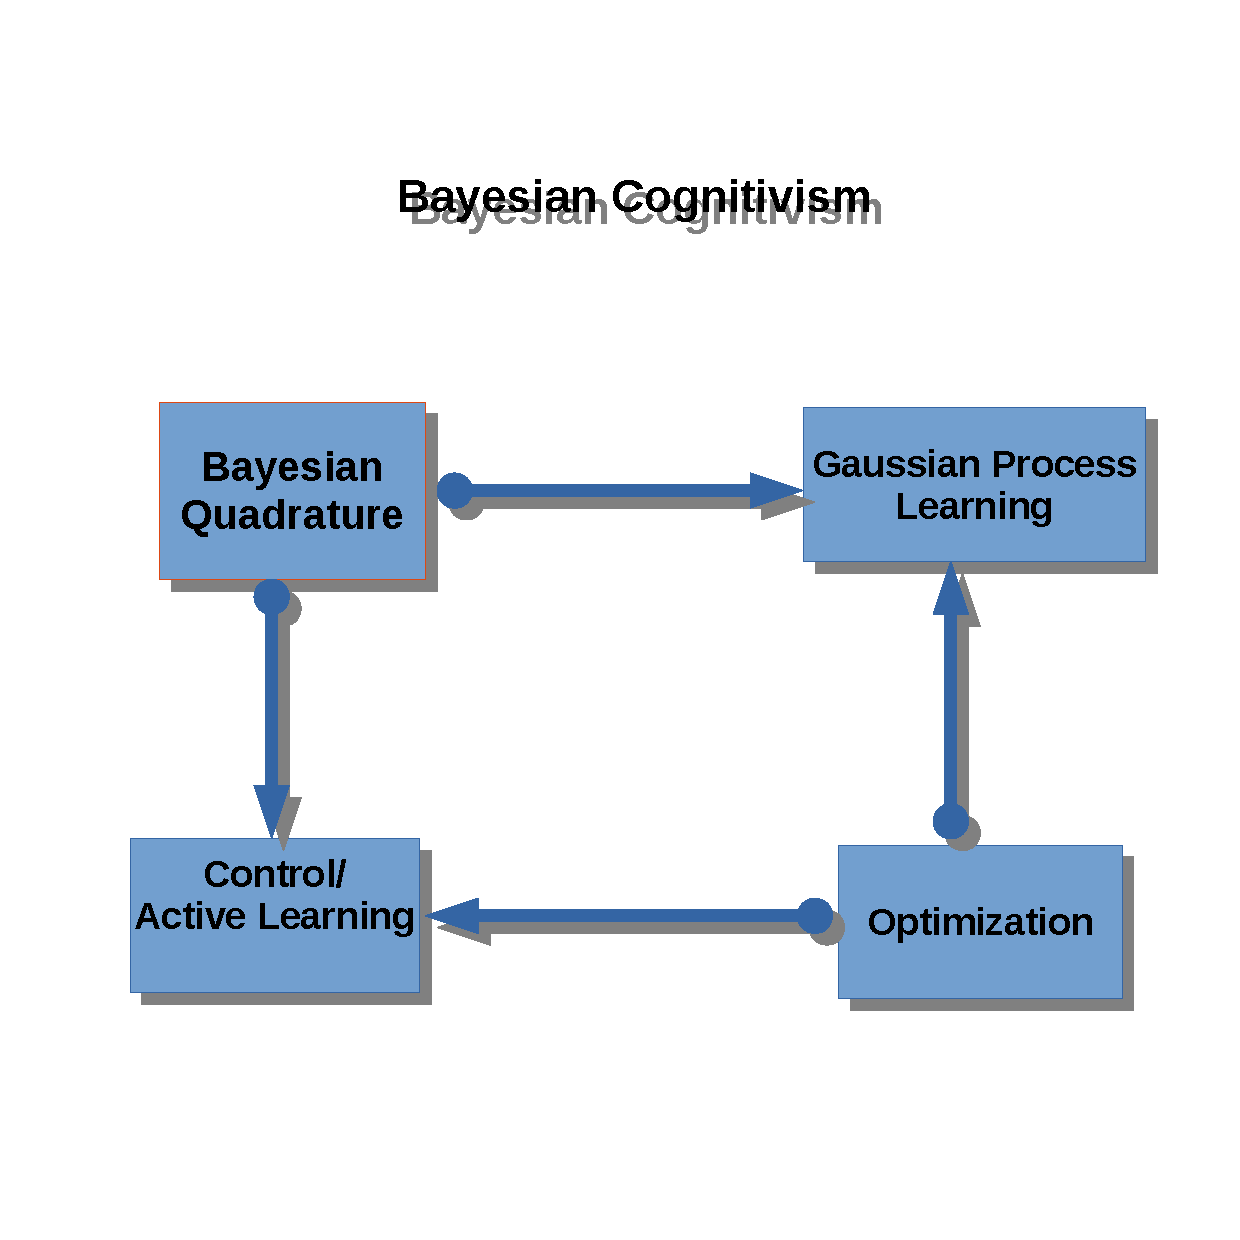
\includegraphics[scale=0.6]{bayescog.pdf}
\end{figure}
\FloatBarrier
The final goal of Bayesian Cognitivism is to model participants behavior as a result of minimizing uncertainty globally and not, as is sometimes done in psychology, locally. If uncertainties can be passed from subparts to subparts easily via posterior calculations of Gaussian Processes, then the global uncertainty reduction hypothesis can be tested directly against local uncertainty reductions. Consider active learning as an example. Current approaches only test for the uncertainty reduction in the \emph{Control} part and are ignorant towards all of the three remaining bits (with the occasional exception of the pure learning part). What the global uncertainty hypothesis predict would be behavior that minimizes uncertainty over all systems, that is an agent should behave in such a way that all 4 parts will experience less uncertainty over time. This could easily be tested by creating scenarios that deliberately disrupt some of the parts individually or a given subset of them combined and testing the predictions against local uncertainty reduction.\medskip\\
However, in order to establish the grand vision of Bayesian Cognitivism as proposed here, we first have to determine the importance of the different subparts, especially the ones that have been by and large neglected by psychology. On such subpart is Quadrature or the integration of unknown functions in order to make sense of different environments. Therefore, we will test in what sense participants can be described by different Quadrature algorithms in the following study.


%%%%%%%%%%%%%%%%%%%%%%%%%%%%%%%%%%%%%%%%%%%%%%%%%%%%%%%%%%%%%%%%%%%%%%%%%%%%%%%%%%%%%%%%%%%%%%%
\chapter{Quadrature}
\emph{This chapter will set up the problem of Quadrature and describe different approaches to solve this problem actively.}

\section{The problem: expectations over functions}
Many problems in Bayesian statistics require us to calculate integrals over unknown functions.
\begin{align}
Z=\int f(x)p(x) dx
\end{align}
Integrals over functions are important for the calculation of expectations, marginal distributions, integrating out nuisance parameters, model comparison, and normalizations, to name but a few problems. In almost any non-trivial situation these functions are normally unknown and might be expensive to assess.\\
As our goal is to come up with a model for how human integrate information in many different situations, we first have to define different ways of how they could do so.
\section{Different Sampling Approaches}
\subsection{Random Walk}
The most simplistic approach towards assessing the area under a function via sampling is to apply sampling completely at random and then to sum up over the observations of the function in question.
\begin{align}
\hat{Z}=\frac{1}{N}\sum_{i=1}^nf(x)
\end{align}
Even though this approach sounds very simplistic it is nonetheless the approach that many psychological theories would propose as the way humans sample both from memory and in their environment.

\subsection{Sequential Bayesian Quadrature}
Bayesian Quadrature tries to approximate the unknown function by the means of Gaussian Process Regression as described above. This method is sometimes described as model-based integration. This approach put a prior on $f$ that is based on a Gaussian Process and then utilizes the fact that a posterior over $f$ implies a posterior over $Z$. In general, the posterior over $Z$ has a mean linear in $f(x_s)$.
\begin{align}
\mathbb{E}[Z|f(x_s)]=\sum_{i=1}^{N}z^{\top}K^{-1}f(x_i)
\end{align}
where $z_n=\int k(x,x_n)p(x)dx$.\\
This approach uses a Gaussian Process as a \emph{surrogate model} for the function $f$ and then assesses the integral via Quadrature over this surrogate model. In its core it is still a passive approach as the inputs are still sampled uniformly from the input $x$. As we intended to find an active learning approach to sampling here, it seems to be natural to consider the variance.
\begin{align}
\mathbb{V}[Z|f(x_s)]=\int \int k(x,x')p(x)p(x')dxdx'-z^{\top}K^{-1}z
\end{align}
It can be shown that an a priori choice to minimize variance would pick all given observation points to be equidistantly, which also matches the common intuition that it is good to cover as much input space as possible if no information was given. However, we are interested in how participants select information sequentially. Therefore, the algorithm we will use to model participants' behavior will try to select observations such that the overall variance will be minimized on each trial. This algorithm is called \emph{Sequential Bayesian Quadrature} and does not put observations into the input space equidistantly, but rather distributes them wisely given some past observations. For example, it would make sense to place more observations into regions where a function shows interesting behavior (i.e. changes more frequently), an intuition captured nicely by the sequential approach.
%%%%%%%%%%%%%%%%%%%%%%%%%%%%%%%%%%%%%%%%%%%%%%%%%%%%%%%%%%%%%%%%%%%%%%%%%%%%%%%%%%%%%%%%%%%%%%%

\chapter{Methods}
\emph{This chapter will provide a detailed description of the used design and recruited participants.}
\section{Participants}
49 participants (26 female, age=18-45) were recruited via prolific academic and received \pounds 1 as a reward.
\section{Design}
Participants were asked to take part in a study about ``frequency distribution'' and it was explained to them that a frequency distributions meant how many out of 1000 randomly sampled people (or events) fulfilled a certain requirement. Participants were presented with 4 different (randomly permuted) scenarios, but the general set up was always the same. First, they were given the problem at hand, for example height. They were then asked to provide a self-assessment, for example ``Please state how tall you are.''. Next, they were told that we had designed an experiment with 1000 trials, in this situation that we had measured the height of 1000 randomly sampled people. Participants were then asked to estimate how many of the sampled people were smaller than them. Afterwards they were shown an empty histogram. This histogram contained the 10 bars of the 1000 sampled people and participants were asked to select 5 bars (out of 10) to appear as wisely as possible in such a way that they could make a better statement about where on the distribution their initial assessment would fall. As we were mostly interested in how participants sample from probability distributions to make integrative judgments, the way they selected information here was the most crucial for our experiment. Lastly, they were allowed to update their initial assessments after they had sampled from the distribution. The exact design of one trial is described in Protocol 1.
\fbox{
\parbox{15cm}{
\begin{enumerate}
\item  Provide personal assessment of value.\vspace{-4mm}
\item Provide cumulative assessment:\\
State how many out of 1000 sample point fall below assessment.\vspace{-4mm}
\item Sample 5 out of 10 bars of histogram sequentially.\vspace{-4mm}
\item Update cumulative assessment.\vspace{-4mm}
\end{enumerate}
}}
\begin{center}Protocol 1: Design of one trial.\end{center}
As we wanted to assess how participants cope with different probability distributions, we chose four different scenarios in 4 different trials using 4 different probability distributions. The first scenario required participants to explore a frequency plot of height which was generated from a normal distribution with $mu=169$ and $\sigma^2=10$.  The second scenario required participants to assess how many emails they receive per day and was generated from a Poisson distribution with $\lambda=8$. The third scenario asked participants to estimated how often one has to roll a dice (on average) until the first 6 appears and thus was generate from a geometric distribution with $p=\frac{1}{6}$. Finally, the last distribution came from a fairly mixed bimodal distribution of two normally distributed variables with $\mathbf{\mu}=[6,10]^\top$ and $\mathbf{\sigma}=[0.7,0.5]^\top$. All probability distributions are depicted in Figure~\ref{dists} below.
\begin{figure}[h!]
\caption{Used probability distributions.}
\label{dists}
  \centering
    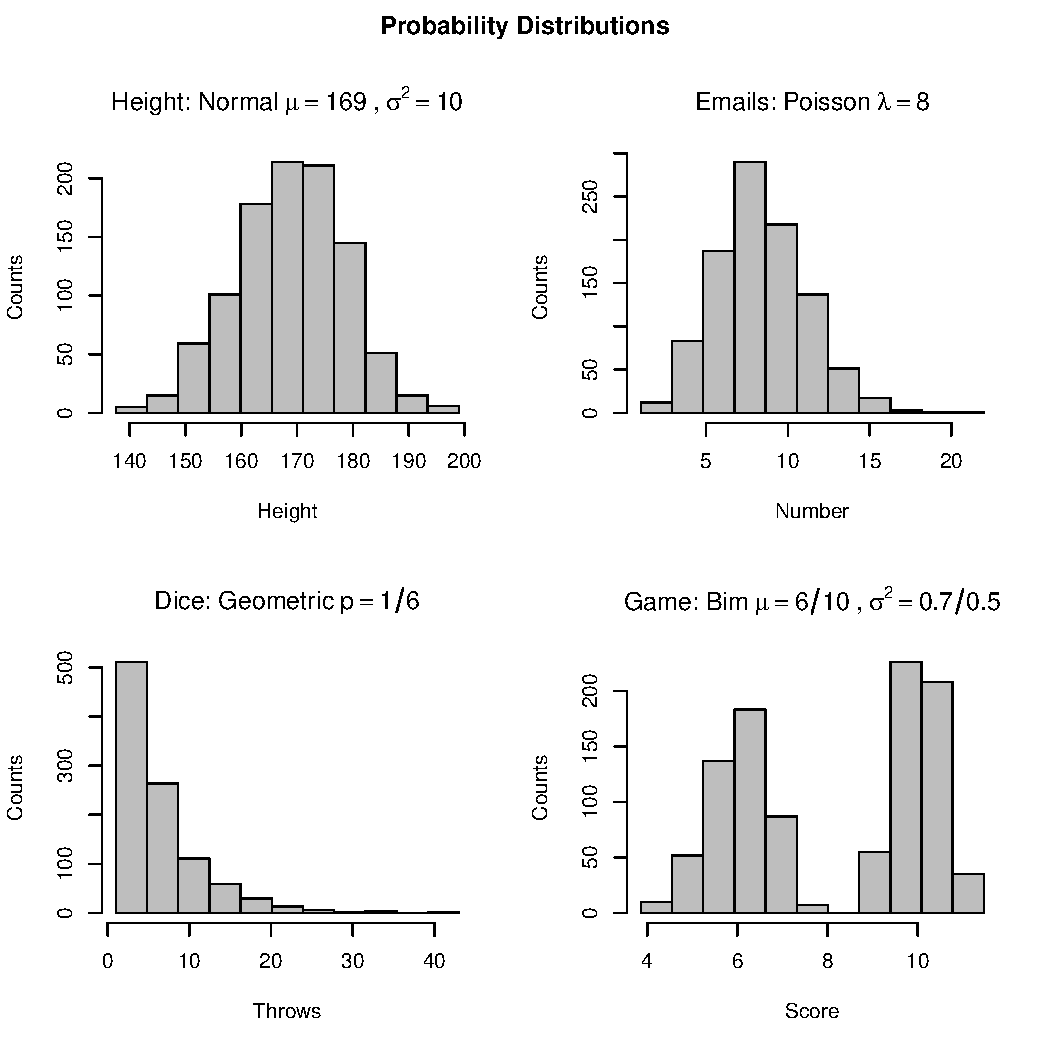
\includegraphics[scale=0.68]{probdists.pdf}
\end{figure}
As said before, the main focus of the experiment was on how participants selected 5 (out of 10) bars, that is ranges, of a frequency plot sequentially. The underlying assumption thereby was that the selection is not random at all, but more likely to follow a Sequential Bayesian Quadrature approach.\\
The experiment was programmed in Javascript/HTML and a screen shot can be seen in Figure~\ref{screenshot} below.
\begin{figure}[h!]
\caption{Used probability distributions.}
\label{screenshot}
  \centering
    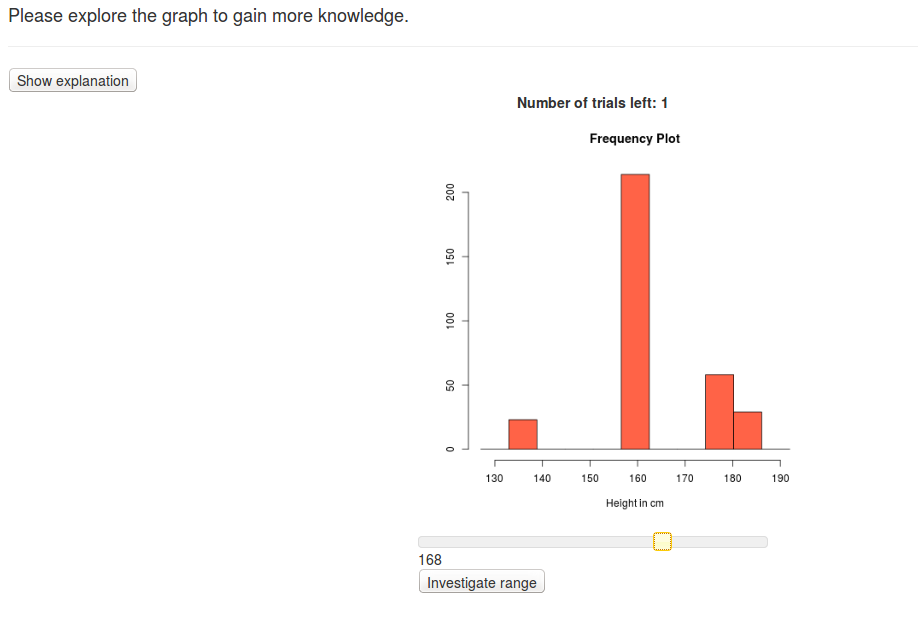
\includegraphics[scale=0.5]{screenshot.png}
\end{figure}
\section{Model comparison approach}
In order to compare the Sequential Bayesian Quadrature approach with the random sampling approach, we calculate the expected reduction in variance for each candidate point $x_{t+1}$ at time point $t$ and evaluated this variance-derived utility by utilizing a simple softmax function.
\begin{align}
\label{softmax}
\sigma(z_{jt}) = \left\{\frac{\exp(z_{jt})}{\sum_{k=1}^{K}\exp(z_{kt})}\right\}
\end{align}
This softmax function then was used to calculate Akaike's ``An Information Criterion'' for each participant, thereby checking how well the Sequential Bayesian Quadrature algorithm described their behavior.
\section{Hypothesis}
Based on the argument above, we hypothesized the following results:
\begin{description}
\item[$\mathcal{H}1$:] Participants' prior assessment will be plausible for cases that they should have intuitive knowledge about.
\item[$\mathcal{H}2$:] Participants' sampling behavior will be non-random and well-described by a Sequential Bayesian Quadrature approach.
\item[$\mathcal{H}3$:]  Participants' posterior assessment will be closer to the truth than their prior assessment. 
\end{description}

%%%%%%%%%%%%%%%%%%%%%%%%%%%%%%%%%%%%%%%%%%%%%%%%%%%%%%%%%%%%%%%%%%%%%%%%%%%%%%%%%%%%%%%%%%%%%%%
\chapter{Results}
\emph{This chapter will show the results of the experiment both in raw and modeled format.}
\section{Raw results}
The input spaces chosen by participants are presented in Figure~\ref{raw} below.
\begin{figure}[h!]
\caption{Used probability distributions.}
\label{raw}
  \centering
    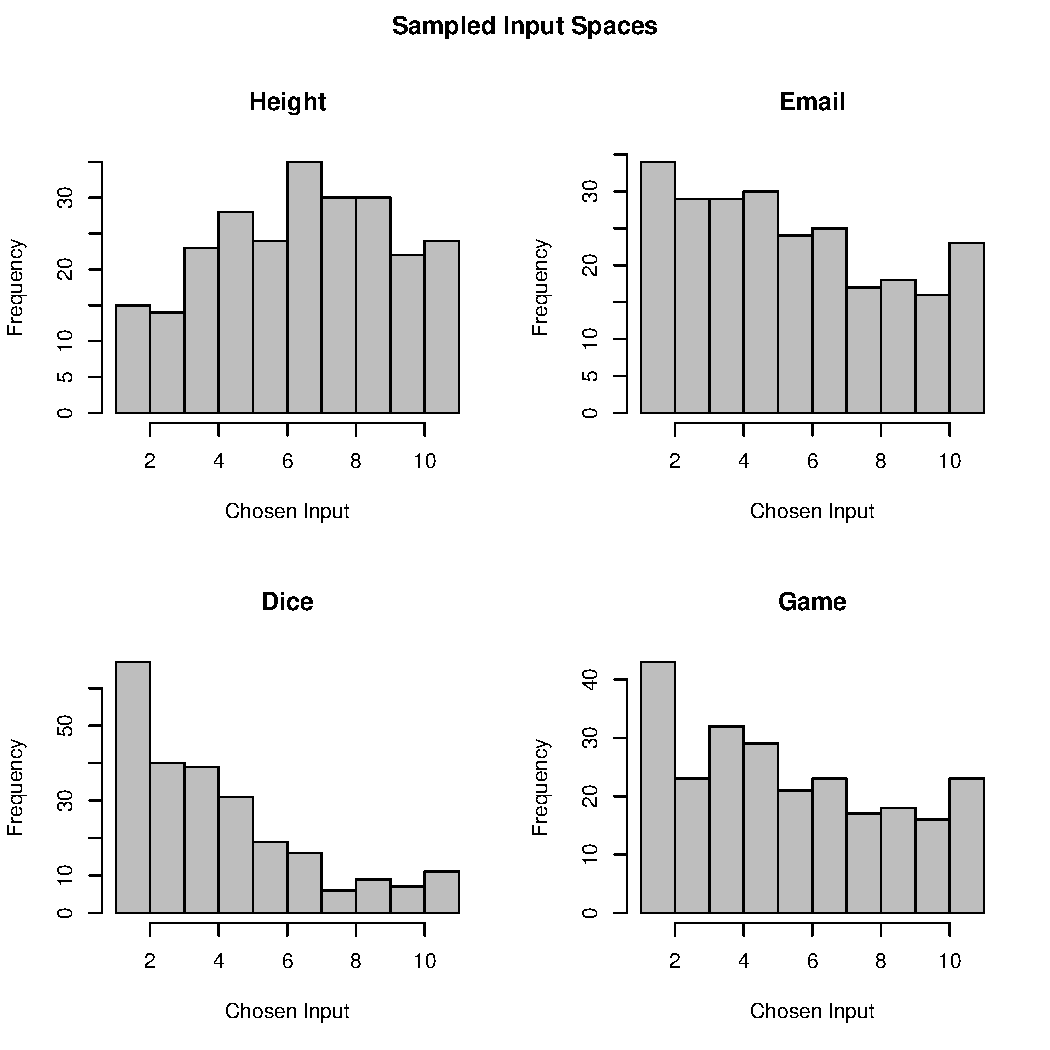
\includegraphics[scale=0.68]{rawsample.pdf}
\end{figure}
It can already be seen that the sampling behavior is not uniform over the whole space, but --at least for the height and the dice example-- seems to match the actual distributional frequencies.\\
Another things to check is the difference between the prior and posterior assessment.  For this, we calculated the true cumulative value, that is --given participants' assessment-- how many of the 1000 trials are expected to be smaller than that value and calculated the distance to that value from their prior and posterior assessment. Results are presented in Figure~\ref{distance}.

\begin{figure}[h!]
\caption{Aggregated distance to truth, prior and posterior.}
\label{distance}
  \centering
    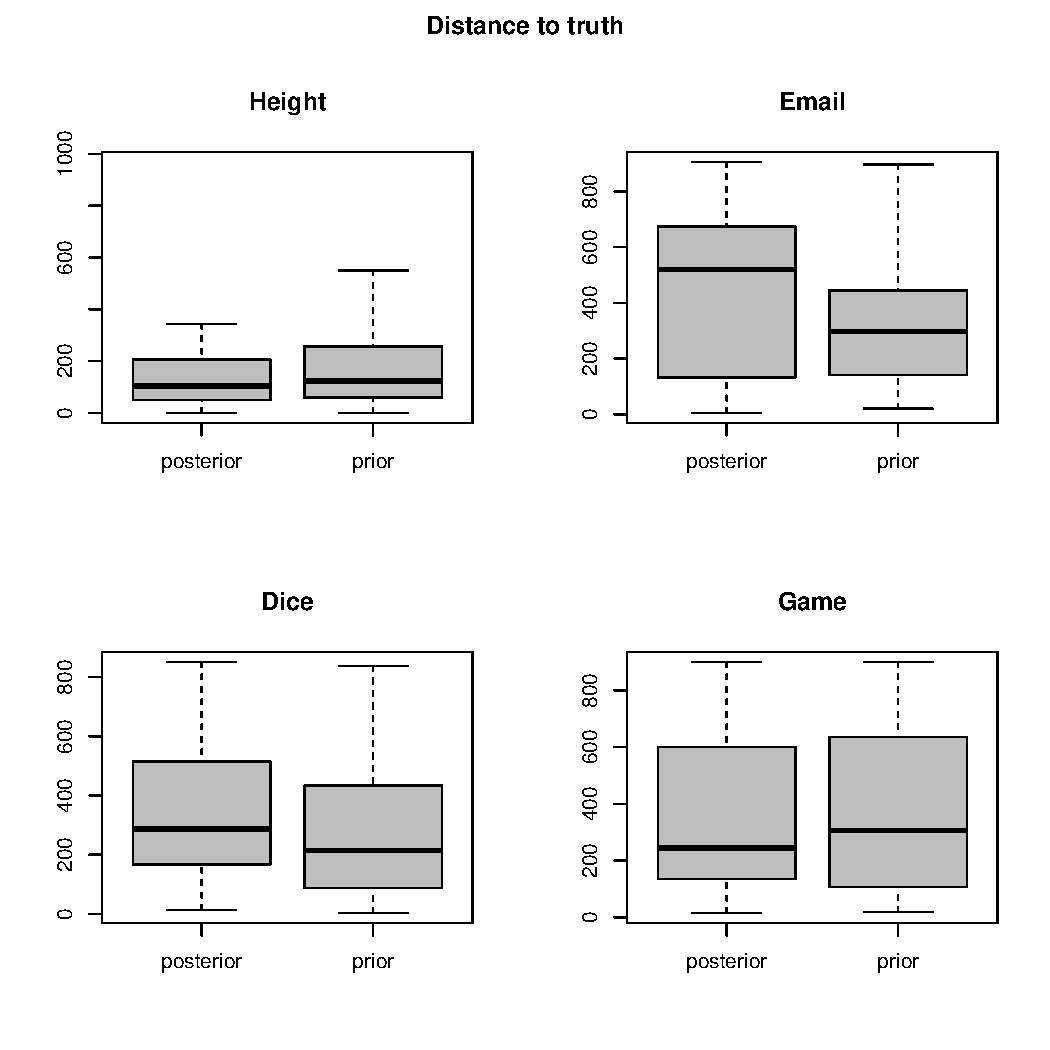
\includegraphics[scale=0.68]{valuedistance.pdf}
\end{figure}
It can be seen that, unfortunately, the posterior assessment only gets better for the height and the game assessment and gets slightly worse for the email and the dice assessment. 

\section{Modeling results}
We checked how well the Sequential Bayesian Quadrature method predicted the one step ahead look-up for each participants for each trial and step and calculated the AIC based on the softmax equation described above. The final modeling results per scenario and participants are shown in Figure~\ref{aic}.
\begin{figure}[h!]
\caption{Used probability distributions.}
\label{aic}
  \centering
    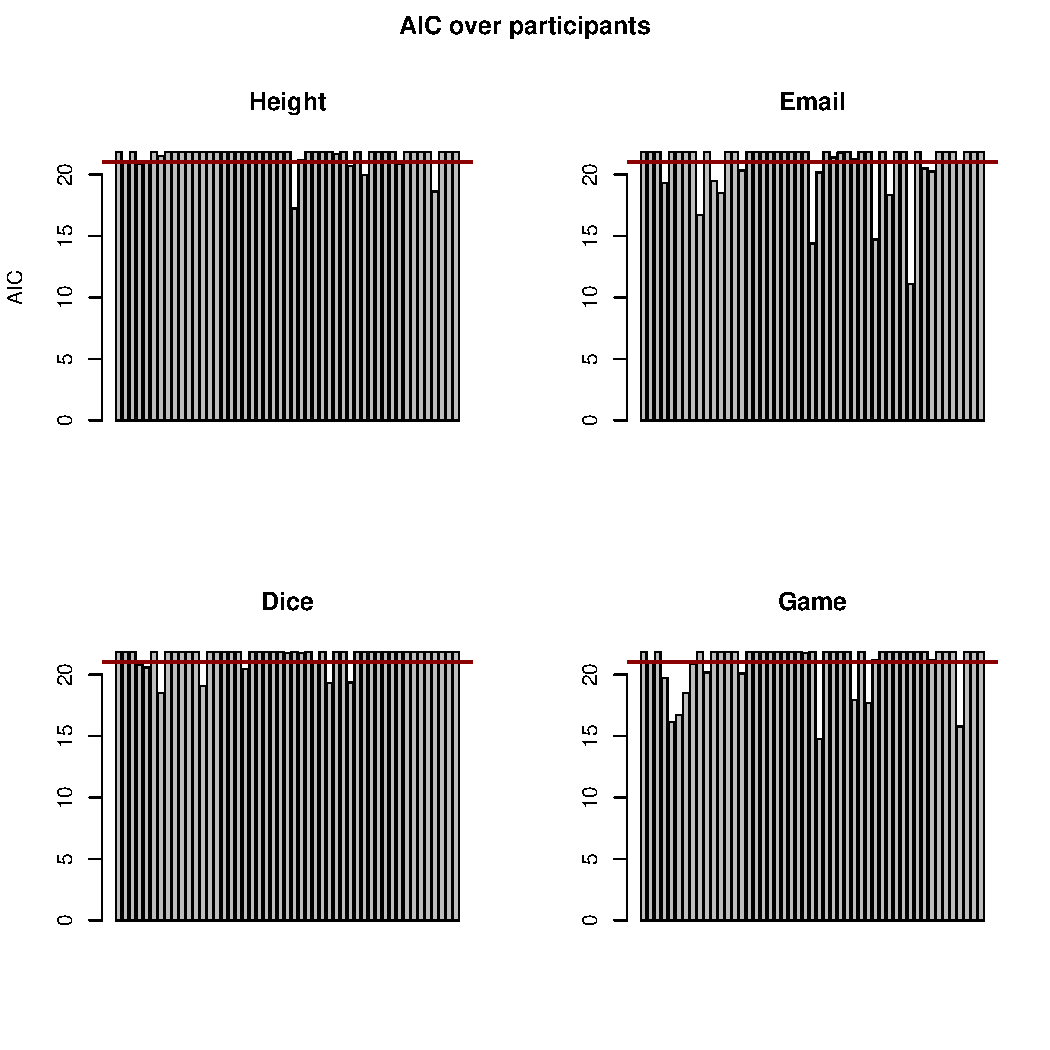
\includegraphics[scale=0.68]{aicbars.pdf}
\end{figure}
Even though not all participants are well-described by the Sequential Bayesian Quadrature approach, the mean AIC-value for all scenarios, height ($t = -3.8661, df = 48, p<0.05$), emails ($t = -3.6799, df = 48, p<0.05$), dice ($t = -4.1012, df = 48, p<0.05$), and game ($t = -4.0018, df = 48, p<0.05$) all differed significantly from the expected mean AIC of a random model. Therefore, the hypothesis that all people sample randomly across the probability space can safely be rejected.
%%%%%%%%%%%%%%%%%%%%%%%%%%%%%%%%%%%%%%%%%%%%%%%%%%%%%%%%%%%%%%%%%%%%%%%%%%%%%%%%%%%%%%%%%%%%%%%
\chapter{Discussion}
\emph{This chapter will discuss the results and explain why the Bayesian Quadrature method outperformed the other methods.}

%%%%%%%%%%%%%%%%%%%%%%%%%%%%%%%%%%%%%%%%%%%%%%%%%%%%%%%%%%%%%%%%%%%%%%%%%%%%%%%%%%%%%%%%%%%%%%%
\chapter{Conclusion}
\emph{This chapter will conclude the thesis by calling for more elaborate assessments of human active sampling.}

\bibliographystyle{apa-good}
{\footnotesize\bibliography{Bibo}}


%%%%%%%%%%%%%%%%%%%%%%%%%%%%%%%%%%%%%%%%%%%%%%%%%%%%%%%%%%%%%%%%%%%%%%%%%%%%%%%%%%%%%%%%%%%%%%%
\end{document}